%% abtex2-modelo-trabalho-academico.tex, v-1.9.2 laurocesar
%% Copyright 2012-2014 by abnTeX2 group at http://abntex2.googlecode.com/
%%
%% This work may be distributed and/or modified under the
%% conditions of the LaTeX Project Public License, either version 1.3
%% of this license or (at your option) any later version.
%% The latest version of this license is in
%%   http://www.latex-project.org/lppl.txt
%% and version 1.3 or later is part of all distributions of LaTeX
%% version 2005/12/01 or later .
%%
%% This work has the LPPL maintenance status `maintained'.
%%
%% The Current Maintainer of this work is the abnTeX2 team, led
%% by Lauro César Araujo. Further information are available on
%% http://abntex2.googlecode.com/
%%
%% This work consists of the files abntex2-modelo-trabalho-academico.tex,
%% abntex2-modelo-include-comandos and abntex2-modelo-references.bib
%%

% ------------------------------------------------------------------------
% ------------------------------------------------------------------------
% abnTeX2: Modelo de Trabalho Academico (tese de doutorado, dissertacao de
% mestrado e trabalhos monograficos em geral) em conformidade com
% ABNT NBR 14724:2011: Informacao e documentacao - Trabalhos academicos -
% Apresentacao
% ------------------------------------------------------------------------
% ------------------------------------------------------------------------

\documentclass[
	% -- opções da classe memoir --
	12pt,				% tamanho da fonte
	openright,			% capítulos começam em pág ímpar (insere página vazia caso preciso)
	oneside,			% para impressão sem verso e anverso. Oposto a twoside
	a4paper,			% tamanho do papel.
	% -- opções da classe abntex2 --
	chapter=TITLE,		% títulos de capítulos convertidos em letras maiúsculas
	%section=TITLE,		% títulos de seções convertidos em letras maiúsculas
	%subsection=TITLE,	% títulos de subseções convertidos em letras maiúsculas
	%subsubsection=TITLE,% títulos de subsubseções convertidos em letras maiúsculas
	% -- opções do pacote babel --
	english,			% idioma adicional para hifenização
%	french,				% idioma adicional para hifenização
%	spanish,			% idioma adicional para hifenização
	brazil				% o último idioma é o principal do documento
	]{abntex2-udesc}

% ---
% Pacotes básicos
% ---
\usepackage{lmodern}			% Usa a fonte Latin Modern
\usepackage[T1]{fontenc}		% Selecao de codigos de fonte.
\usepackage[utf8]{inputenc}		% Codificacao do documento (conversão automática dos acentos)
\usepackage{lastpage}			% Usado pela Ficha catalográfica
\usepackage{indentfirst}		% Indenta o primeiro parágrafo de cada seção.
\usepackage{color}				% Controle das cores
\usepackage{graphicx}			% Inclusão de gráficos
\usepackage{microtype} 			% para melhorias de justificação
\usepackage{mathptmx}
% ---

% ---
% Pacotes de citações
% ---
%\usepackage[brazilian,hyperpageref]{backref}	 % Paginas com as citações na bibl
\usepackage[alf,abnt-emphasize=bf,abnt-etal-cite=2]{abntex2cite}	% Citações padrão ABNT
%,abnt-full-initials=yes
%\citeoption{abnt-and-type=&}

% ---
% Pacotes de cor em tabela
% ---
\usepackage[table]{xcolor}
\usepackage{array,ragged2e}

% ---
% Pacotes de algoritmos
% ---
\usepackage{listings}
% ---
% CONFIGURAÇÕES DE PACOTES
% ---

% ---
% Configurações do pacote backref
% Usado sem a opção hyperpageref de backref
%\renewcommand{\backrefpagesname}{Citado na(s) página(s):~}
% Texto padrão antes do número das páginas
%\renewcommand{\backref}{}
% Define os textos da citação
%\renewcommand*{\backrefalt}[4]{
%	\ifcase #1 %
%		Nenhuma citação no texto.%
%	\or
%		Citado na página #2.%
%	\else
%		Citado #1 vezes nas páginas #2.%
%	\fi}%
% ---% ---
% Configurações do pacote listings
\lstdefinelanguage{portugol}
  {morekeywords={Algoritmo,Var,inteiro,Inicio,escreva,Fim}
}
\lstset{
  breakatwhitespace=false,
  breaklines=true,
  keywordstyle=\bfseries\color{black},
  language=portugol,
  showstringspaces=false,
}
% ---% ---

% ---
% Informações de dados para CAPA e FOLHA DE ROSTO
% ---
\titulo{Interpretador de Algoritmos Portugol em HTML5}
\autor{Gilberto Tavares}
\cidade{São Bento do Sul}
\uf{SC}
\local{\inserecidade, \insereuf}
\data{2016}
\orientador{Dr. Luiz Cláudio Dalmolin}
\instituicao{Universidade do Estado de Santa Catarina - UDESC}
\centro{Centro de Educação do Planalto Norte - CEPLAN}
\curso{Bacharelado em Sistemas de Informação}
\tipotrabalho{Trabalho de Conclusão de Curso}
% O preambulo deve conter o tipo do trabalho, o objetivo,
% o nome da instituição e a área de concentração
\preambulo{Trabalho de Conclusão apresentado ao Curso de Bacharelado em Sistemas
de Informação, da Universidade do Estado de Santa Catarina, como requisito para
a obtenção do grau de Bacharel em Sistemas de Informação}
% ---

% ---
% Configurações de aparência do PDF final

% alterando o aspecto da cor azul
%\definecolor{blue}{RGB}{41,5,195}
\definecolor{blue}{rgb}{0,0,0}

% informações do PDF
\makeatletter
\hypersetup{
     	%pagebackref=true,
		pdftitle={\@title},
		pdfauthor={\@author},
    	pdfsubject={\imprimirpreambulo},
	    pdfcreator={LaTeX with abnTeX2},
		pdfkeywords={lógica da programação}{algoritmos}{portugol}{interpretador}{html5},
		colorlinks=true,       		% false: boxed links; true: colored links
    	linkcolor=black,          	% color of internal links
    	citecolor=blue,        		% color of links to bibliography
    	filecolor=magenta,      		% color of file links
		urlcolor=blue,
		bookmarksdepth=4
}
\makeatother
% ---

% ---
% Espaçamentos entre linhas e parágrafos
% ---

% O tamanho do parágrafo é dado por:
\setlength{\parindent}{1.3cm}

% Controle do espaçamento entre um parágrafo e outro:
\setlength{\parskip}{0.2cm}  % tente também \onelineskip

% ---
% compila o indice
% ---
\makeindex
% ---

% ----
% Início do documento
% ----
\begin{document}
% Retira espaço extra obsoleto entre as frases.
\frenchspacing

% ----------------------------------------------------------
% ELEMENTOS PRÉ-TEXTUAIS
% ----------------------------------------------------------
% \pretextual

% ---
% Capa
% ---
% TODO PRINT Descomentar
%\imprimircapa
% ---

% ---
% Folha de rosto
% (o * indica que haverá a ficha bibliográfica)
% ---
%\imprimirfolhaderosto*
% TODO PRINT Descomentar
%\imprimirfolhaderosto
% ---

% Folha de Aprovação
% TODO PRINT Descomentar
%
% ---
% Inserir folha de aprovação
% ---

% Isto é um exemplo de Folha de aprovação, elemento obrigatório da NBR
% 14724/2011 (seção 4.2.1.3). Você pode utilizar este modelo até a aprovação
% do trabalho. Após isso, substitua todo o conteúdo deste arquivo por uma
% imagem da página assinada pela banca com o comando abaixo:
%
% \includepdf{folhadeaprovacao_final.pdf}
%
\begin{folhadeaprovacao}

  \begin{center}
    {\ABNTEXchapterfont\bfseries\MakeTextUppercase{\imprimirautor}}

    \vspace*{\fill}\vspace*{\fill}
    \begin{center}
      \ABNTEXchapterfont\bfseries\MakeTextUppercase{\imprimirtitulo}
    \end{center}
    \vspace*{\fill}

   \end{center}

  \noindent
  \imprimirpreambulo

  \vspace*{\fill}

  \noindent
  {\bfseries Banca Examinadora}

  \vspace*{\ABNTEXsignskip}

  \setlist[description]{font=\normalfont}

  \begin{description}[labelindent=0pt,labelwidth=4cm] %label={\textnormal},
    \item[Orientador:]
    \assinaturaorientador{\textbf{\href{http://lattes.cnpq.br/7393306373465290}{\imprimirorientador} \\ Universidade do Vale do Itajaí}}
  \end{description}

  \setlist[description]{font=\bfseries}

  \begin{description}[labelindent=0pt,labelwidth=4cm] %label={\textnormal},
    \item[Membros:]
    \vspace*{\ABNTEXsignskip}
    \assinaturaorientador{\textbf{\href{http://lattes.cnpq.br/3985354928735296}{Dr. Nilson Ribeiro Modro} \\ Universidade Federal de Santa Catarina}}
    \item[]
    \vspace*{\ABNTEXsignskip}
    \assinaturaorientador{\textbf{\href{http://lattes.cnpq.br/3317225251677148}{Ma. Nelcimar Ribeiro Modro} \\ Universidade Federal do Paraná}}
  \end{description}

   \begin{center}
    \vspace*{0.5cm}
    \inserecidade~\insereuf, 29/11/2016
    \vspace*{1cm}
  \end{center}

\end{folhadeaprovacao}
% ---


% Dedicatória, Agradecimentos, Epígrafe - Elementos Pré textuais opcionais
% TODO PRINT Descomentar
%
% Dedicatória

% ---
% Dedicatória
% ---
\begin{dedicatoria}
   \vspace*{\fill}
   \hspace{.45\textwidth}
   \begin{minipage}{.5\textwidth}
      \SingleSpacing
Dedico este aos meus familiares falecidos:
% Talvez reticências ...

Meu irmão que sempre apoiou minha formação
superior e carreira até oferecendo certa
colaboração financeira.

E ainda mais recente meu pai que financiou
meu pré ingresso e não pude compartilhar
com ele esta conquista.
   \end{minipage}
	\vspace*{\fill}
\end{dedicatoria}
% ---


% ---
% Agradecimentos
% ---
\begin{agradecimentos}

A minha mãe me apoiou em minha decisão de cursar faculdade em outra cidade. E
sempre que possível, mesmo com dificuldade, ajudou como pode com móveis para meu
primeiro quarto, algumas compras e mercado e algum dinheiro quando ficava mais
crítico. Inclusive isso tudo pode ter sido um dos motivos da decisão dela em
vender o imóvel em morávamos.

A toda a família Lischka que me acolheu inicialmente como hóspede na residência
do casal Arnaldo e Jacira (prima da minha mãe). Foi também na empresa familiar
deles juntos com seus filhos que tive meu primeiro emprego na cidade e me cedido
para moradia o quartinho e dependências junto à empresa.

Ao meu irmão que me empregou as sábados e minhas cunhadas que me hospedavam, além de amigos. A todos os motoristas que me deram carona, econominanzo assim a parassagem para que eu pudesse voltar com uma grana a mais do final de semana.

A Joseli que sua experiência passando pelo mesma situação de fim de curso foi de grande ajuda. Também seu apoio e motivação, bem como dos meu amigos de infância José e Rafael que fizeram o mesmo.

A toda a experiência social, esportiva e de conheciento que as confraternizações com outros academicos, Jiudesc e os vários Latinoware proporcionaram.

Sem esquecer é claro das minhas garrafas térmicas, que mantiveram tanto café quentinho ou suco de guaraná gelado para embalar as noites dedicadas a esta realização.


\end{agradecimentos}
% ---

% Epígrafe

% ---
% Epígrafe
% ---
\begin{epigrafe}
    \vspace*{\fill}
   \hspace{.45\textwidth}
   \begin{minipage}{.5\textwidth}
      \SingleSpacing

% No idioma de origem
% ``Most good programmers do programming not
% because they expect to get paid or get adulation
% by the public, but because it is fun to program..''

% Tradução original
% ``A maioria dos bons programadores programam não
% porque esperam ser pagos ou adulados pelo público,
% mas porque é divertido programar.''

{\small``A maioria dos bons programadores programa
não por esperar ser pago ou adulado pelo público,
mas porque é divertido programar.''  (tradução nossa)

\vspace{\onelineskip}

Linus Torvalds}
   \end{minipage}
	\vspace*{\fill}
\end{epigrafe}
% ---



% Resumos (em português e pelo menos em inglês)
% TODO PRINT Descomentar
%
% ---
% RESUMOS
% ---

% resumo em português
\begin{resumo}
Trata-se do estudo das opções para prática computacional no processo de ensino e aprendizagem, sugerindo um conceito de ferramenta que diferente das existentes permite acesso via navegador de internet sem instalação ou download mesmo que apenas de complementos ou já disponíveis no computador. Vários conceitos são apresentados sobre algoritmos sua estrutura e seus "transformadores", sejam eles compiladores, tradutores ou interpretadores. Mas para o foco do trabalho apenas instruções simples de escrita em tela sem utilização de variáveis foi utilizada, permitindo demonstrar seu diferencial que além de acesso via navegador, nativamente (diferindo das demais soluções similares), o acesso mesmo sem conexão com a internet.

\vspace{\onelineskip}
\textbf{Palavras-chaves}: Lógica da programação. Algoritmos. Portugol. Interpretador. HTML5.
% ensino, aprendizagem
\end{resumo}

% resumo em inglês
%\begin{resumo}[Abstract]
%\begin{otherlanguage*}{english}
%
%\vspace{\onelineskip}
%\textbf{Key-words}: Programming logic. Algorithms. Portugol. Interpreter. HTML5.
%% teaching, learning
%\end{otherlanguage*}
%\end{resumo}


% Lista de Siglas
% TODO PRINT Descomentar
%
% ---
% inserir lista de abreviaturas e siglas
% ---
\begin{siglas}
  \item[CSS] Hyper Text Markup Language
  \item[HTML] Hyper Text Markup Language
  \item[UNESA] Universidade Estácio de Sá
\end{siglas}
% ---


% ---
% inserir o sumario
% ---
\pdfbookmark[0]{\contentsname}{toc}
\tableofcontents*
\cleardoublepage
% ---



% ----------------------------------------------------------
% ELEMENTOS TEXTUAIS
% ----------------------------------------------------------
\textual

% ----------------------------------------------------------
% Introdução (exemplo de capítulo sem numeração, mas presente no Sumário)
% ----------------------------------------------------------
\chapter{Introdução}
%\addcontentsline{toc}{chapter}{Introdução}
% ----------------------------------------------------------


A base da programação é ensinar máquina a realizar determinada tarefa. Para isso
pode-se dizer que independente do paradigma utilizado no processo de
desenvolvimento ele envolve algoritmos.

Algoritmos podem não necessariamente serem computacionais, já que são um
conjunto de passos finitos. Analogias simplistas são os ingredientes e modo de
preparo de uma receita ou interiores para uma tarefa do cotidiano como a troca
de um pneu furado em um automóvel.

Porém se tratando de computação deve ter maior exatidão seguindo uma linguagem
pois diferente do ser humano uma máquina não é tão interpretativa.
Desconsideradas aqui inteligências artificiais que são desenvolvidas por
algoritmos para terem  comportamento de compreensão humana. Isto pode ser
analogamente algo como não entender idioma estrangeiro e as instruções estarem
nesta linguagem. Porém em informática isso tem que ser mais especificado com
palavras ou caracteres predeterminados de início e fim, de blocos, repetições,
etc.

Sendo o berço mais popular da informática os Estados Unidos da América e seus
criadores em muitos casos dessa origem ou de países com mesmo idioma as
primeiras linguagens de computação e a maioria delas são em inglês.

Isso muda quando falamos do Portugol que possui variações, mas resumidamente
sua origem vem como uma tradução de uma linguagem de programação simples e comum
com seus termos em nosso idioma nativo no Brasil, pela nossa colonização
portuguesa.

Tendo como foco o aprendizado de algoritmos para uma boa fundamentação de
futuros programados ou profissionais da área, e muitas vezes a facilidade com
o inglês não é algo comum nosso país, a linguagem em Portugol de torna um
artifício vantajoso.

% TODO Analisar necessidade de reecrista, remoção, relocação
O que se propõe aqui em ter ferramenta de aprendizado composta de editor de
texto para a escrita dos algoritmos e visualizador do resultado dos mesmo.
E que não seja necessária instalação, seja facilmente acessível como qualquer
outra página web em computadores ou dispositivos móveis e mesmo assim permaneça
acessível mesmo sem conexão disponível com a internet.

% TODO Analisar necessidade de reecrista, remoção, relocação
Este projeto visa demonstrar que um novo interpretador para a pseudolinguagem
Portugol, que tem o propósito de facilitar o estudo da lógica de programação vem
ao encontro como solução para muitas dificuldades atuais no âmbito de
aprendizagem acadêmica. Para tal, seguiu-se a ideia de implementar este
interpretador, onde haverá a preocupação em desenvolvê-lo seu protótipo em dois
módulos: Interpretador e Interface Homem-Máquina além de sugir um Sistema de
Informação para o Professor. Essa ferramenta é um interpretador para a
pseudolinguagem Portugol, gratuito e com uma interface adequada.


\section{Objetivos do Trabalho}

\ifdraft{\color{green}}{}\subsection{Objetivo Geral}

Apresentar o conceito de ferramenta computadorizada para se tornar referência
em criação, edição, visualização e interpretação de algoritmos em
pseudolinguagem, como alternativa às existentes. Sendo seu diferencial o acesso
nativo a partir de navegadores \textit{Web} modernos. Inclusive acessível
quando uma conexão com a internet esteja indisponível.
% NOTE \footnote{Desde que haja ao menos um acesso anterior.}

\subsection{Objetivos Específicos}

Visando atingir o objetivo geral em sua totalidade lista-se a seguir objetivos
específicos de modo sucinto:

\begin{itemize}
\setlength\itemsep{0em}

\item Desenvolver o protótipo, sendo seu código fonte aberto e
disponível para que outros possam manter, ampliar e evoluir a aplicação;

\item Fazê-lo compatível com a sintaxe desenvolvida na Universidade Estácio
de Sá (UNESA) a UNESA \textit{Algorithmic Language} (UAL). E mínimo produto
viável para a primeira lição de ensino aprendizagem;

\item Permitir o acesso via navegadores \textit{Web} modernos, sem
necessidade de instalações complementares;

% Para isso utilizar HTML5 que pode ser descrito como o uso de somente linguagem de programação ECMAScript (popularmente Javascript), e para inferface gráfica essencialmente a combinação de HTML (abreviação para a expressão inglesa HyperText Markup Language, que significa Linguagem de Marcação de Hipertexto) e de estilização em Cascading Style Sheets (CSS) em suas versões recomendáveis pelo World Wide Web Consortium (W3C).

\item Aplicar aprimoramentos introduzidos na versão 5 da
\textit{HyperText Markup Language} (HTML) para uso sem conexão com a
internet.

\end{itemize}\color{black}


\section{Justificativa do Trabalho}

No processo de ensino ao invés de abstração em papel, utilizar prática em software auxilia e muito o aproveitamento na aprendizagem. Em algoritmos é necessário o pensamento lógico, em alguns casos o aluno vêm com deficiência inclusive em lógica geral. ``O Aprendizado de algoritmos não é uma tarefa muito fácil, só se consegue através de muitos exercícios'' \cite[p.~1]{lopes2002etal}. Para esse ensino é essencial conhecer dois conceitos principais: lógica de programação e algoritmos. Primeiramente é apresentado um paralelo de situações do cotidiano com algoritmos, ao efetuar comparações de instruções passo a passo realizadas diariamente, como fritar um ovo ou trocar um pneu de automóvel.

Após o entendimento básico da lógica, passa-se então para o uso de uma ferramenta computacional para a simulação destes algoritmos, aplicando descrição na linguagem estruturada em português. Em alguns casos, utiliza-se de linguagens em inglês, como por exemplo, Pascal. Há professores que preferem usar pseudo linguagem em português somente ``em papel'', iniciando a codificação diretamente em linguagem C. Tem-se inclusive, também ``em papel'', de analisar e interpretar os passos do algoritmo para saber quais serão os valores em memória e a saída na tela.

Simultaneamente, com a prática escrita, sem software específico, pode-se simular os mesmos algoritmos em interpretador ou compilador. Sendo em um interpretador sua construção dividida em partes, cada uma com uma função específica. Geralmente identifica-se: o analisador léxico, o analisador sintático, o analisador semântico, e o resultado de saída. Caso seja um compilador há, ao invés de resultado de saída, o gerador de código, que transforma o programa em linguagem de máquina composta de 0s e 1s \cite{delamaro2004}.

Diante do exposto, este trabalho justifica-se pelo empenho em facilitar o processo de aprendizagem de algoritmos, desenvolvendo um programa em navegador via Internet, fazendo com que seja desnecessária a instalação do programa,  podendo ser acessado a partir de qualquer computador, com o objetivo que os exercícios sejam resolvidos com maior praticidade.\color{black}


\section{Estrutura do Trabalho}


No presente trabalho apresentar-se-á a forma de desenvolvimento do primeiro
módulo, o interpretador, a interface com o usuário e diretrizes para a
execução do módulo restante que não será executado, e que poderão ser ampliados
a partir desta base de estudo e conhecimentos aplicados no presente projeto.

O restante do projeto está organizado da seguinte forma: no capítulo 2 é
relatada a forma como foi idealizado o desenvolvimento da ferramenta proposta;
no capítulo 3 descreve-se como o módulo interpretador está sendo desenvolvido;
nos capítulos 4 e 5 são apresentadas as diretrizes que serão seguidas para os
desenvolvimentos dos módulos Interface Homem-Máquina e sugestão de Sistema de
Informação para o Professor, respectivamente; no capítulo 5 são apresentados as
considerações finais.


% Capítulo 2
\chapter{Fundamentação Teórica}

Para o entendimento e desenvolvimento de trabalho, alguns conceitos teóricos devem ser dispostos. Por exemplo o \textbf{Processamento de Linguagem Natural} (PLN) que tem menor rigidez do que se faz necessário para uma máquina, onde conjuntos de instruções podem ser descritos de modo humanamente mais natural \cite{medina2006etal}. Exemplificando esse processamento de linguagem tem-se um conversa explicando uma rota para determinado destino ou uma receita culinária. Os demais conceitos presentes neste capítulo são algoritmos, tradutores e algumas ferramentas com proposta de prática computacional de algoritmos, no aprendizado de lógica da programação.

\section{Programa de Computador}

%\textrightarrow
Como explica \citeonline{Santana2016} programas de computador \textit{Command-Line Interface} (CLI), tem sua interação através de um \textit{Shell} (BASH, DOS, entre outros). Este tipo de programa é contrário à \textit{Graphical User Interface} (GUI), que possui interação visual. A estrutura de um programa de computador de tipo CLI é E$\,\to\,$P$\,\to\,$S (entrada-programa-saída), podendo não haver argumentos de entrada. Por exemplo, um programa pode receber em sua execução, como argumento, um número inteiro para resultar em sua raiz quadrada. Outro programa já ter em seu código um número pré definido para o mesmo cálculo.

\section{Pseudo código ou linguagem}

Pseudocódigos são estruturados a partir de um idioma e utilizados como \textit{Program Design Language} (PDL), que permite descrição escrita de algoritmos com flexibilidade na estrutura. No entanto com utilização de pseudocódigo, menos alternativas são possíveis em um mesmo algoritmo. Portugol é um pseudocódigo que tem aplicabilidade no ensino de lógica da programação, desde \citeonline{saliba1992} confirma-se sua utilização para este fim. Buscando aproximar de linguagens de programação, criaram-se a partir do Portugol algumas variação de pseudolinguagem. Não há contudo um consenso na padronização, porém sensíveis são as semelhanças entre as variações. Para formalidade nos pseudo códigos ou linguagens, foi criado o inglês estruturado, que tem sua origem na linguagem de programação Pascal. Certamente outros idiomas tem suas versões, mas no caso de Portugal, Brasil e outros países de mesma origem utilizam o português estruturado denominado Portugol.

\section{Algoritmos}

A última das notas de Ada Lovelace, que foram republicadas em 1953\nocite{1253887}, apresenta os primeiros conceitos sobre programação, descrevendo um algoritmo. Desde então estes foram difundidos, sendo utilizados até a atualidade. Algoritmo é um termo mais amplo, sendo inclusive destinado a outras áreas e finalidades além da programação \cite{medina2006etal}.

As definições de algoritmo encontradas na literatura são interpretativas, porém todas chegam ao mesmo resultado, um \textbf{conjunto de instruções para a resolução de uma situação}. Sendo esta a definição de algoritmo, pode então ele representar um programa de computador, apresentando operações e instruções específicas para a saída que se pretende. A Tabela \ref{tab:structsalgo} apresenta as estruturas representáveis em um algoritmo, de acordo com \citeonline{santiago2003etal}.

%Alguns autores afirmam que estas instruções mas afirmações são determinam instruções são passos detalhadas para a solução ou mesmo que tipo de situação, se especificamente um problema ou tarefas em geral.
%Como podemos perceber, um programa nada mais é que um tipo de algoritmo. Sua particularidade é que suas operações são específicas para o computador e restritas ao conjunto de instruções que o processador pode executar. Podemos considerar esse conjunto de instruções como a primeira linguagem de programação do computador, também chamada de linguagem de máquina.

\begin{table}[ht]
\centering
  \caption{Estruturas representáveis em algoritmos}\label{tab:structsalgo}
\begin{tabular}{ l | l }\hline
\textbf{Estrutura} & \textbf{Descrição} \\ \hline
Tipos de dados & Tipo de valores inserido nas variáveis. \\ \hline
Variáveis & Armazenagem na memória principal. \\ \hline
Atribuições & Definir valor numa variável. \\ \hline
Operações aritméticas & Utilizadas em cálculos entre números e variáveis. \\ \hline
Operações relacionais & Estabelecem relação entre comparações. \\ \hline
Estruturas de controle & Para fluxo, com desvio condicional e laços de repetição. \\ \hline
Vetores & Variáveis com único nome, contendo um índice de posições. \\ \hline
Matrizes & Semelhante a vetores, porém de dimensão dupla. \\ \hline
Funções & Subprogramas com ou sem passagem de parâmetro.
\end{tabular}
  \caption*{\footnotesize Fonte: Produção do autor, 2016.}
\end{table}

% Com base nos dois parágrafos abaixo, reescrever utilizado como referência de embasamento os autores \cite{santiagodazzi2003}
%Um algoritmo consiste em um procedimento, composto por uma série de passos
%utilizados para resolver problemas computacionais específicos, que a partir do
%processamento comdados de entradas irá gerar dados de saídas (CORMEN et al,
%1999).
%Para efetuar funcionalidade em um algoritmo e verificar a integridade deste é
%necessário testar o algoritmo verificando o conteúdo das variáveis passo a
%passo. Para efetuar esta tarefa costuma-se utilizar o Teste de Mesa. Também
%chamado Teste Exaustivo, executa para cada instrução, uma verificação, e a
%amostragem do conteúdo das variáveis utilizadas no algoritmo, permitindo que o
%programador visualize o comportamento de todo o processo. Isso permite não
%apenas a comprovação do correto funcionamento, mas também detectar e corrigir
%com facilidade eventuais erros.

\section{Tradutores}
%Compiladores e Interpretadores

%Um compilador traduz um programa descrito em uma linguagem de alto nível, mais
%adequada aos seres humanos, para os códigos em uma linguagem de máquina, que
%podem ser executados por um processador. Grosso modo, o processo de
%compilação pode ser descrito como contendo as seguintes etapas: análise léxica, análise
%sintática, análise semântica e geração de código.\cite{barbosa2009etal}

No âmbito da computação, tradutor é um programa que traduz uma linguagem de programação para outra equivalente. Conforme \citeonline{aho2007etal} existem dois principais tipos de tradutores: compiladores e interpretadores. A diferença entre Compilador e Interpretador pode ser compreendida na Figura \ref{fig:versus}, o interpretador na execução traduz diretamente cada instrução, partindo os dois de um mesmo código fonte.

\begin{figure}[h]
  \caption{Diferença de Compilador e Interpretador}\label{fig:versus}
  \centering
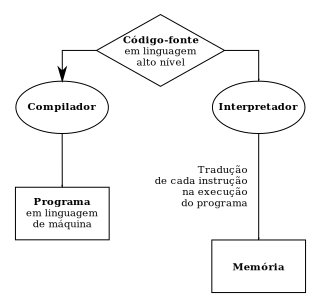
\includegraphics[width=.75\textwidth,keepaspectratio]{figures/compilador-interpretador.pdf}
  \caption*{\footnotesize Fonte: Produção do autor, adaptado de \citeonline{medina2006etal}.}
\end{figure}

Passando por um processo de entendimento de elementos mínimos no código, ignorando outros e agrupando em símbolos especificados, a compilação se inicia. Além dessa análise também é necessária a verificação se esses grupos estão em ordem ou outros erros possíveis. \citeonline{delamaro2004} descreve que código fonte de entrada termina tendo como saída o programa objeto, o compilador converte a linguagem simples em uma linguagem entendida pela máquina. Na Figura \ref{fig:compilador} é possível visualizar um compilador, somente com a principal etapa e dela as análises: Léxica, Sintática e Semântica.

\begin{figure}[h]
  \caption{Análises de um compilador}\label{fig:compilador}
  \centering
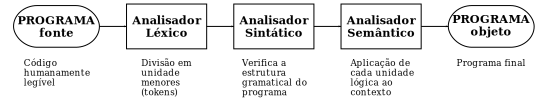
\includegraphics[width=.98\textwidth,height=10cm,keepaspectratio]{figures/etapas-compilador.pdf}
  \caption*{\footnotesize Fonte: Produção do autor, adaptado de \citeonline{ferrandin2005etal}.}
\end{figure}

\subsection{Processo de compilação}

Num compilador ideal, de acordo com \citeonline{aho2007etal} e visto na Figura \ref{fig:fullcompiler}, pode-se identificar a etapa de \textbf{análise} (\textit{front end}) e a etapa de \textbf{síntese} (\textit{back end}). Na síntese a partir da árvore sintática são geradas representações intermediárias até o programa alvo executável através de: geração de código intermediário, otimização de código e por fim o gerador de código. Durante todo o processo a tabela de símbolos guarda informação sobre nomes declarados e o tratamento de erros que age na etapa de análise, por exemplo, identificando erro e em qual linha.

\begin{figure}[h]
  \caption{Compilador completo}\label{fig:fullcompiler}
  \centering
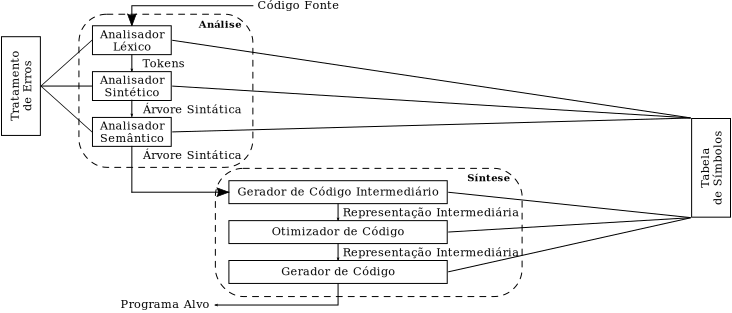
\includegraphics[width=\textwidth,keepaspectratio]{figures/compilador-completo.pdf}
  \caption*{\footnotesize Fonte: Produção do autor, adaptado de \citeonline{aho2007etal}.}
\end{figure}

%\subsection{Análise Morfológica}
%
\subsection{Análise Léxica}

A análise léxica (\textit{scanner}) é citada por \citeonline{aho2007etal} como sendo onde elementos mínimos (\textit{tokens}) são identificados, cada letra, número e outros caracteres (como pontuação e demais símbolos), além do espaço. Após reconhecidos, esses \textit{tokens} são então agrupados em lexemas: identificadores, palavras-chave reservadas, comandos, operadores, constantes, conjunto de texto, nome de variáveis, início e fim do algoritmo ou de blocos. Essa análise também ignora comentários e marcas de edição (tabulações, caracteres de avanço de linha e espaços). No Quadro \ref{qua:print} é dado uma linha do algoritmo para na Tabela \ref{tab:lexemas} apresenta os lexemas identificados.

\begin{quadro}[h]
\centering
  \caption{Exemplo para entendimento de tradutor}\label{qua:print}
\begin{lstlisting}[language=ual,frame=single]
  imprima "Aprendendo Algoritmo";
\end{lstlisting}
  \caption*{\footnotesize Fonte: Produção do autor, 2016.}
\end{quadro}

\begin{table}[h]
\centering
  \caption{Lexemas encontrados no exemplo preposto}\label{tab:lexemas}
\begin{tabular}{ c | l }\hline
\textbf{Lexema} & \textbf{Classificação} \\ \hline
\texttt{imprima} & identificador da expressão de impressão \\ \hline
\texttt{"Aprendendo Algoritmo"} & conjunto literal de texto \\ \hline
\texttt{;} & caractere de encerramento de expressão \\ \hline
\end{tabular}
  \caption*{\footnotesize Fonte: Produção do autor, 2016.}
\end{table}

\subsection{Análise Sintática}

Análise sintática (\textit{parser}), recebe a sequência de lexemas da análise anterior e determina se são elementos estruturais pertencentes à linguagem desejada, exposto por \citeonline{delamaro2004}. Esses elementos são estruturados de modo ramificado (Figura \ref{fig:ast}), dando origem ao termo árvore sintática. São essas estruturas: expressões aritméticas, comandos de atribuição ou declarações de procedimentos e as relações entre eles, garantindo que seja correto sintaticamente.

\begin{figure}[h]
  \caption{Exemplo de árvore sintática}\label{fig:ast}
  \centering
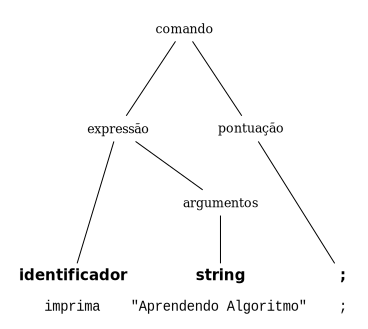
\includegraphics[width=.4\textwidth,height=10cm,keepaspectratio]{figures/ast.pdf}
  \caption*{\footnotesize Fonte: Produção do autor, 2016.}
\end{figure}

\subsection{Análise Semântica}

A análise semântica verifica o ``significado'' de comandos, ao tratar de aspectos relacionados a sua ordem para que tenha sentido dentro do definidido pela gramática da linguagem para a correta execução. É possível que um programa esteje em acordo com a sintáxe gramatical, porém apresente erros quanto a semântica. A gramática da linguagem é definida por uma árvore gramatical (\textit{tree grammar}), é utilizada nesta etapa. Por exemplo se só for possível imprimir conjuntos literais de texto, variáveis, conjuntos dessas ou operações aritméticas entre parênteses e for criado como impressão direta de um número.

\section{Ferramentas Existentes}
% Ferramentas para prática de algoritmos

\begin{itemize}

\item \textbf{ILA + AMBAP}: Desenvolvida por \citeonline{evaristo2000} o Interpretador de Linguagem Algorítmica (ILA) é um intepretador via linha de comando no qual o AMBAP - AMBiente para Aprenzidadeo e Programaçao utitilizou em seu editor.

\item \textbf{UAL + EditorUAL}: Desenvolvido por \citeonline{spallanzani2000etal} na UNESA era basicamente compilador via linha de comando, desenvolvido em Haskel para linux. Ele foi posteriormente portado para Windows, e neste recebeu um editor próprio.

\item \textbf{VisuAlg}: Desenvolvida por Claudio Morgado de Souza profissional programador e analista bem como professor universitário, é utilizada tanto em cursos técnicos quanto em meio universitário. A facilidade de obtenção do seu executável para Windows (não necessária instalação), documentação e simplicidade, sem perder funções úteis para iniciantes, são grandes atrativos \cite{souza2013etal}.

\item \textbf{Web Portugol}: Desenvolvida por pesquisadores na UNIVALI permite o acesso via navegadores que tenham integração com Java, desde que o mesmo também esteja instalado no computadors \cite{souza2013etal}.

\item \textbf{Construtor}: Desenvolvido pelo Centro Educacional de Informática Aplicada do SENAC (Rio de Janeiro), é a primeira encontrada para uso em Windows e tem a vantagem acompanhar o livro ``Construção de Algoritmos'' de \citeonline{fernandes1999etal}.

\end{itemize}

Na Tabela \ref{qua:compare-tools} consta exposto um comparativo de pontos que ressaltam como fatores determinantes em escolha de qual opção utilizar pelo educador no ensino para que seus alunos pratiquem o conteúdo.

\begin{table}[h]
\centering
\caption{Comparativo das ferramentas}\label{qua:compare-tools}
\resizebox{\textwidth}{!}{%
\begin{tabular}{ r | l | l | l | l | l }\hline
& UAL+Editor & ILA+AMBAP & VisuAlg & Web Portugol & Contrutor \\ \hline
Plataforma & Linux e Windows & DOS/Windows & Windows & Web (Java Applet) & Windows \\ \hline
Licença & \textit{open source} & \textit{freeware} & \textit{freeware} & \textit{open source} & \textit{open source} \\ \hline
Instituição & UNESA & UFAL &  & UNIVALLI & SENAC \\ \hline
Linguagem & Haskell & Java (editor) &  & Java & \\ \hline
\end{tabular}%
}
  \caption*{\ifdraft{\color{green}}{}\footnotesize Fonte: Produção do autor.}
\end{table}

Desenvolvida por \citeonline{esmin1998} quando vinculado a UNOESC o \textbf{Portugol/Plus} é a mais antiga opção encontrada no Brasil. Merecendo destaque por ser comumente referenciada por outros autores, inclusive quando tratam sobre desenvolvimento de novas soluções. Porém por ser em plataforma \textit{Disk Operating System (DOS)}, inclusive com interface gráfica foi desconsiderada no levantamento acima.

Ao delimitar a quantidade de itens outras também não foram listadas, alguns casos o acesso ao programa para testes não estava disponível ou menor relevância na literatura. No entanto  merecem menção: \textbf{PascalX}, por Athur Vargas Lopes da ULBRA; \textbf{Web-UNERJOL}\nocite{ferrandin2005etal}, utilizando UNERJOL os dois pelo mesmo acadêmico na UNERJ com colaborações distintas.
%PascalX\nocite{http://www.ulbra.tche.br/~avl/home.htm}

Outras mais não foram consideradas por fugirem do escopo ao utilizar robótica, jogos, foco em estrutura de dados ou similares: Guido VanRobot, Robot Prog, Kids Ruby, Fut Code, TBC-AED. Eram pretendidas somente ferramentas com pseudo-linguagem algorítmica em português, preferencialmente Portugol, partindo novamente do Editor UAL como referencial.
%TBC-AED: por pesquisadores da Universidade Federal de Lavras/Departamento de Ciências da Computação em Minas Gerais

\section{Caso de Ensino com Livro e Ferramenta}

O livro ``Introdução à programação: 500 algoritmos resolvidos'' de \citeonline{lopes2002etal} tem um grande apelo por seu elevado número resoluções como seu título deixa claro. Isso motiva os educadores utilizarem como livro texto base de disciplinas de ensino de Lógica da Programação. Neste livro todos os algoritmos propostos para execução computadorizada estão impressos na sintexe UAL - variante do Portugol - acompanha mídia ótica que contém os exercícios nesta e também em ILA. Na Tabela \ref{tab:compare-ualila} é visto a comparação entre elas.

%\the\textwidth
%455.0pt
%\halftextwidth
%227.7pt
%\noindent
\begin{table}[h]
\centering
  \caption{Comparação entre UAL e ILA}\label{tab:compare-ualila}
\begin{tabular}{p{75mm} | p{75mm}}\hline
\multicolumn{1}{c|}{\textbf{Em UAL}} & \multicolumn{1}{c}{\textbf{Em ILA}} \\ \hline
\begin{lstlisting}[language=ual,style=table]
prog algoritmo11
  imprima "Aprendendo Algoritmo!!!";
fimprog
\end{lstlisting} &
\begin{lstlisting}[language=ila,style=table]
//prog algoritmo11
inicio
  limpar
  escrever "Aprendendo Algoritmo!!!"
fim
\end{lstlisting} \\ \hline
\end{tabular}
  \caption*{\ifdraft{\color{green}}{}\footnotesize Fonte: Produção do autor, a partir dos exemplos de \citeonline{lopes2002etal}.}
\end{table}

Todo o projeto está pautado neste algoritmo simplista, obtido em \citeonline[p.~26]{lopes2002etal} e na mídia que acompanha o livro destes autores. Facilmente se nota a diferença nos blocos de início e fim do programa, além de somente em UAL ter o nome do mesmo (solucionado com uso de linha comentada) e o comando de limpeza somente necessário em ILA. As chamadas de escrita em tela também têm sua palavra reservada diferente. Nenhuma delas delimita o argumento por parênteses e UAL exige ponto e vírgula ao final. As duas não são sensíveis no uso de letras maiúsculas ou minúsculas nas palavras chaves .

\begin{table}[h]
\centering
  \caption{Escopo das linguagens UAL e ILA}\label{tab:escopo-lang}
\begin{tabular}{lC{40pt}|C{40pt}}
\cline{2-3}
 & \textbf{UAL} & \textbf{ILA} \\ \hline
\multicolumn{1}{l|}{Saída em tela} & \textbf{s}im & \textbf{s}im \\ \hline
\multicolumn{1}{l|}{Entrada de argumentos} & \textbf{s}im & \textbf{s}im \\ \hline
\multicolumn{1}{l|}{Tipos de dados} & \textbf{s}im & \textbf{s}im \\ \hline
\multicolumn{1}{l|}{Variáveis} & \textbf{s}im & \textbf{s}im \\ \hline
\multicolumn{1}{l|}{Atribuições} & \textbf{s}im & \textbf{s}im \\ \hline
\multicolumn{1}{l|}{Operações aritiméticas} & \textbf{s}im & \textbf{s}im \\ \hline
\multicolumn{1}{l|}{Operações relacionais} & \textbf{s}im & \textbf{s}im \\ \hline
\multicolumn{1}{l|}{Estruturas de controle} & \textbf{s}im & \textbf{s}im \\ \hline
\multicolumn{1}{l|}{Vetores} & \textbf{s}im & \textbf{s}im \\ \hline
\multicolumn{1}{l|}{Matrizes} & \textbf{n}ão & \textbf{s}im \\ \hline
\multicolumn{1}{l|}{Funções} & \textbf{n}ão & \textbf{s}im \\ \hline
\end{tabular}
  \caption*{\ifdraft{\color{green}}{}\footnotesize Fonte: Produção do autor, baseado em \citeonline{spallanzani2000etal,evaristo2000}.}
\end{table}

Sendo as estruturas de um algoritmo o escopo da linguagem, há diferenças entre UAL e ILA também quando quanto sua abrangência, visto Tabela \ref{tab:escopo-lang} sendo a primera estrutura única que o presente trabalho abrange. Não tendo a UAL estruturas como matrizes n-dimensionais, funções com ou sem passagem de parâmetros, novos comandos para tomada de decisões e controle de repetições, novos tipos de dados, conversores de tipos \cite{spallanzani2000etal}.

\ifdraft{}{
%\subsection{Ensino Aprendizagem}

% NOTE citar Teoria das Inteligências Múltiplas de Gardner

%\section{Pseudoliguagem e Portugol}


%
%
%
%
%
%\item G-Portugol
%
%\item Portugol IDE
%
%\item Portugol Studio
%
%\item ASA
%
%\item ATMUF
%
%\item AWTM
%
%\item AMBAP
%
%\item CIFluxProg
%
%\item RAFF
%
%\item SistLog
%
%\item Ambiente SICAS
%
%\item C-Tutur
%
%\item PL-Detective

%\end{itemize}

%\subsection{UAL e Editor UAL}

%\subsection{Demais Aplicativos}
%
%%\subsection{Plataforma Digitais de Ensino}
%\subsection{Ambiente Virtual de Aprendizagem - AVA}
%
%% NOTE Interactive Learning - Aprendizado Interativo {tonin2012etal}
%
%\subsubsection{Udacity}
%
%\subsubsection{Codeacademy}
%
%\subsubsection{SoloLearn}
%
%\subsubsection{Code School}
%
%\subsubsection{Kan Academy}
%
%\subsection{Programação em Blocos}
%
%\subsubsection{\textit{Blockly}}
%
%\section{\textit{Online Judge}}
%
%Sistema de Apoio a Competições de Programação é a denominação em português de
%\textit{Online Judge} por \citeonline{campos2004etal}, nomeado como BOCA.
%E mais recente foi desenvolvido por acadêmico da URI (Universidade Regional
%Integrada do Alto Uruguai e das Missões) com base nesse trabalho anterior o URI
%\textit{Judge Online} \cite{tonin2012etal}.
%
%\section{Tecnologias Web}
%
%\subsection{Linguagem de Marcação de Texto}
%
%\subsection{Liguagem de Programação para Web}
%
%\subsubsection{ECMAScript}
%
%\subsubsection{WebAssembly}
%
%\subsection{Navegadores Web}
%
%\subsection{Aprimoramentos para Uso \textit{Offline}}
}



%% ----------------------------------------------------------

%% ELEMENTOS POS-TEXTUAIS

\postextual

\bibliographystyle{abntex2-alf}
\bibliography{refs}

\end{document}
